% Shared paper body. Included by main.tex (anonymous, for review) and
% main_named.tex (named preprint). Edit the paper here, once.

\begin{abstract}
Prognostics for unmanned-aircraft engines is usually posed as regression of remaining useful life (RUL) in hours. We examine that target with a physics-grounded shadow twin of a turbocharged four-cylinder aero piston engine, which turns multivariate 1~Hz telemetry into residuals at the measured operating point, and a simulated run-to-failure fleet with stochastic faults, manufacturing scatter and realistic instrumentation. Privileged-information oracles show that the target is largely unpredictable: a regressor given the simulator's hidden wear state reaches only 0.77 of the label's standard deviation~($\sigma$), and a sensor-only LSTM already reaches 0.80$\sigma$, because faults that arrive after the prediction time dominate the remaining error. We therefore reframe prognostics as the calibrated probability of failure within dispatch-relevant horizons, and let the system abstain: it publishes a horizon only where it has measured skill and never shows operators an uncalibrated hours estimate. A gradient-boosted classifier with out-of-fold isotonic calibration attains engine-grouped ROC-AUC 0.89--0.92 and Brier skill 0.40--0.46 at 25--100~h, with expected calibration error between 0.007 and 0.020 at 12--100~h on held-out engines, and its loss of skill toward 400~h is reported per horizon instead of being hidden in an average. For sub-limit anomaly detection, the same twin runs a three-tier detector whose fusion rule lets two agreeing models raise a caution while no certified limit is crossed, but never an emergency; on 40 held-out engines it reaches precision 0.996 at a 0.95\% false-positive rate. On real NGAFID piston-aircraft maintenance data, the same per-flight features reach ROC-AUC 0.76--0.77.
\end{abstract}

\section{Introduction}

Medium-altitude long-endurance (MALE) unmanned aircraft typically fly on a single small piston engine with an endurance of 12 hours or more, so an in-flight engine failure usually means losing the aircraft. Maintenance of these engines is still driven by fixed intervals, with inspections every 100 flight hours and overhaul at a manufacturer-set time between overhauls (TBO), and by certified operating limits that trip only once a parameter is already out of range. Prognostics and health management (PHM) promises earlier, condition-based decisions, and its dominant formulation is regression of remaining useful life (RUL), popularised by the C-MAPSS turbofan benchmark \citep{saxena2008damage,zheng2017lstm,li2018dcnn,lei2018review}.

A regressor always returns a number of hours. Whether that number carries information is a separate question, and on real fleets it is hard to answer because the true degradation state is never observed. A physics-based simulator changes this: because it generates the degradation, it can also train \emph{oracles} with privileged access to the hidden state and measure how much of the RUL variance is predictable at all.

We build such a setting for a turbocharged, fuel-injected four-cylinder aero piston engine (Rotax 915~iS) and use it to ask what a prognostic system for this engine class should predict. Our answer is that it should not predict hours. Faults arrive at random after the prediction time and change the rate of decline, so even an oracle that sees the complete hidden wear state leaves most of the RUL variance unexplained, and a sensor-only model is already within 5\% of that oracle. The question that does have an answer is \emph{whether} the engine will fail within a horizon, not \emph{when}: how likely is it to fail within the next $H$ flight hours? It is also the question a dispatcher actually asks.

Our contributions are:
\begin{itemize}
\item A measured argument, based on privileged-information oracles over a physics-based run-to-failure fleet, that point RUL in hours is dominated by aleatoric uncertainty for this engine class (Section~\ref{sec:rul}).
\item Abstaining prognostics: a reformulation as calibrated failure-horizon classification with out-of-fold isotonic calibration, under which the system abstains on any horizon without measured Brier skill and never publishes an uncalibrated hours estimate, evaluated on held-out engines (Section~\ref{sec:surv}).
\item A safety-gated three-tier fusion rule that repairs a defect in the reference specification, under which models could never raise an alert while limits were silent, and keeps emergencies rule-confirmed. For sub-limit detection, it flags 6,567 of the 7,558 degraded windows on which every certified limit is still satisfied, at precision 0.996 (Section~\ref{sec:det}).
\item An evaluation discipline of engine-grouped splits, enforced leakage guards and external checks on real NGAFID flights and on C-MAPSS, with every number reported together with its protocol (Section~\ref{sec:ext}).
\end{itemize}
All fault data in this paper are simulated; we are not aware of any public run-to-failure dataset for UAV piston engines. The external checks therefore test the method, not the deployed model.

\begin{figure*}[t]
\centering
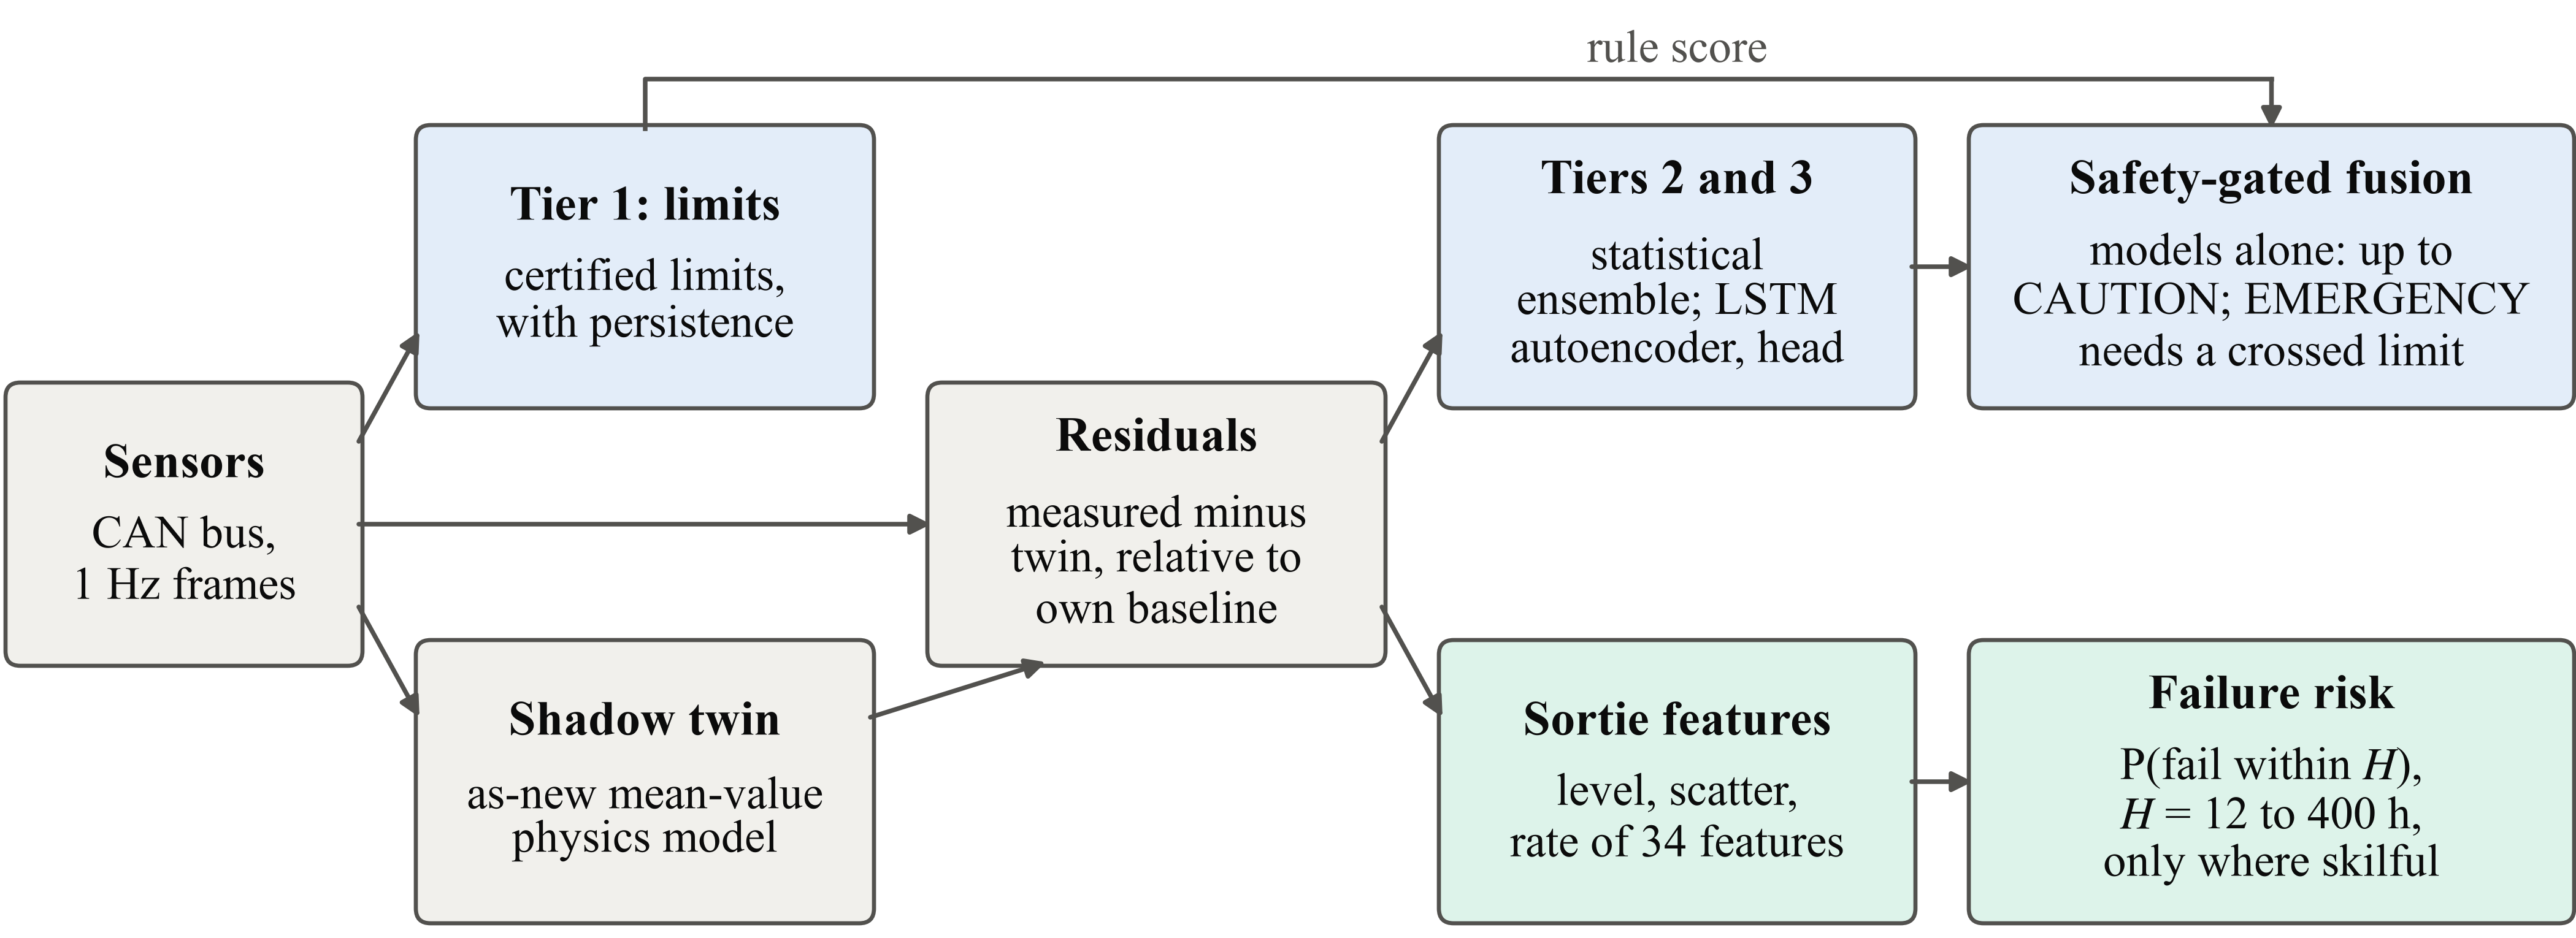
\includegraphics[width=\textwidth]{figures/fig_pipeline.png}
\caption{The digital twin. A physics-based shadow twin, held at as-new condition, turns sensor readings into residuals relative to each engine's own early-life baseline. The detection lane fuses certified limits with two model tiers; the prognostics lane aggregates each sortie and outputs calibrated failure probabilities per horizon.}
\label{fig:pipeline}
\end{figure*}

\section{Related Work}

\noindent\textbf{Remaining useful life.} Data-driven RUL estimation is surveyed by \citet{si2011review} and \citet{lei2018review}. On C-MAPSS \citep{saxena2008damage}, recurrent \citep{zheng2017lstm} and convolutional \citep{li2018dcnn} networks trained on windows with a piecewise-linear capped target became standard, and \citet{saxena2010metrics} introduced prognostic metrics such as $\alpha$-$\lambda$ accuracy and relative accuracy that judge estimates near end of life rather than on average. Most work reports RMSE against a target whose predictability is never quantified; we measure it directly.

\noindent\textbf{Survival and calibration.} Time-to-event models, from proportional hazards \citep{cox1972} to deep competing-risks networks such as DeepHit \citep{lee2018deephit}, treat failure as a probability over time. Modern classifiers are often miscalibrated \citep{guo2017calibration}; isotonic regression \citep{zadrozny2002isotonic} is a standard non-parametric remedy, and the Brier score \citep{brier1950} is a strictly proper scoring rule \citep{gneiting2007proper}. We combine per-horizon classifiers with out-of-fold isotonic calibration and gate what operators see on Brier skill.

\noindent\textbf{Digital twins and anomaly detection.} A digital twin pairs an asset with a model that runs alongside it \citep{tao2019twin}, and physics-informed machine learning uses such models to inform learning \citep{karniadakis2021piml}. We use a mean-value engine model \citep{hendricks1990mvem,heywood1988} as an as-new reference and learn from its residuals. Our statistical tier combines Isolation Forest \citep{liu2008iforest}, CBLOF \citep{he2003cblof} and the matrix profile \citep{yeh2016matrix}; the deep tier uses an LSTM \citep{hochreiter1997lstm} autoencoder in the style of \citet{malhotra2016lstmed}. Because flawed benchmarks have created an illusion of progress in time-series anomaly detection \citep{wu2023flawed}, we score only held-out engines and exclude, rather than assign, windows whose label is ambiguous.

\noindent\textbf{Aviation maintenance on real data.} \citet{yang2022ngafid} predicted unplanned maintenance on general-aviation piston aircraft from NGAFID flight records with convolutional transformers, and \citet{yang2022dataset} released a benchmark subset that we use as our real-data check. Our evaluation practice follows the leakage taxonomy of \citet{kapoor2023leakage}.

\section{System and Data}
\label{sec:system}

\noindent\textbf{Shadow twin.} The twin (Figure~\ref{fig:pipeline}) is a mean-value model of the engine, comprising atmosphere, air path, turbocharger with wastegate, combustion with pre-computed flame properties, and a lumped thermal model with airframe cooling flaps, advanced at a fixed time step. Every parameter carries a source tag (type-certificate data, operator's manual, or derived). Held at as-new condition, it predicts what a healthy engine would show at the current operating point, and the residual between measurement and twin is the main input to every learned component. Residuals matter because the engine's control loops hide degradation from the raw channels: in our model a 30\% radiator blockage raises coolant temperature by only 1.9\,$^\circ$C, far below its 120\,$^\circ$C limit, because the cooling flaps open from 49\% to 68\% of their travel to compensate, a shift the twin registers on the first sortie (Figure~\ref{fig:cooling}).

\begin{figure}[t]
\centering
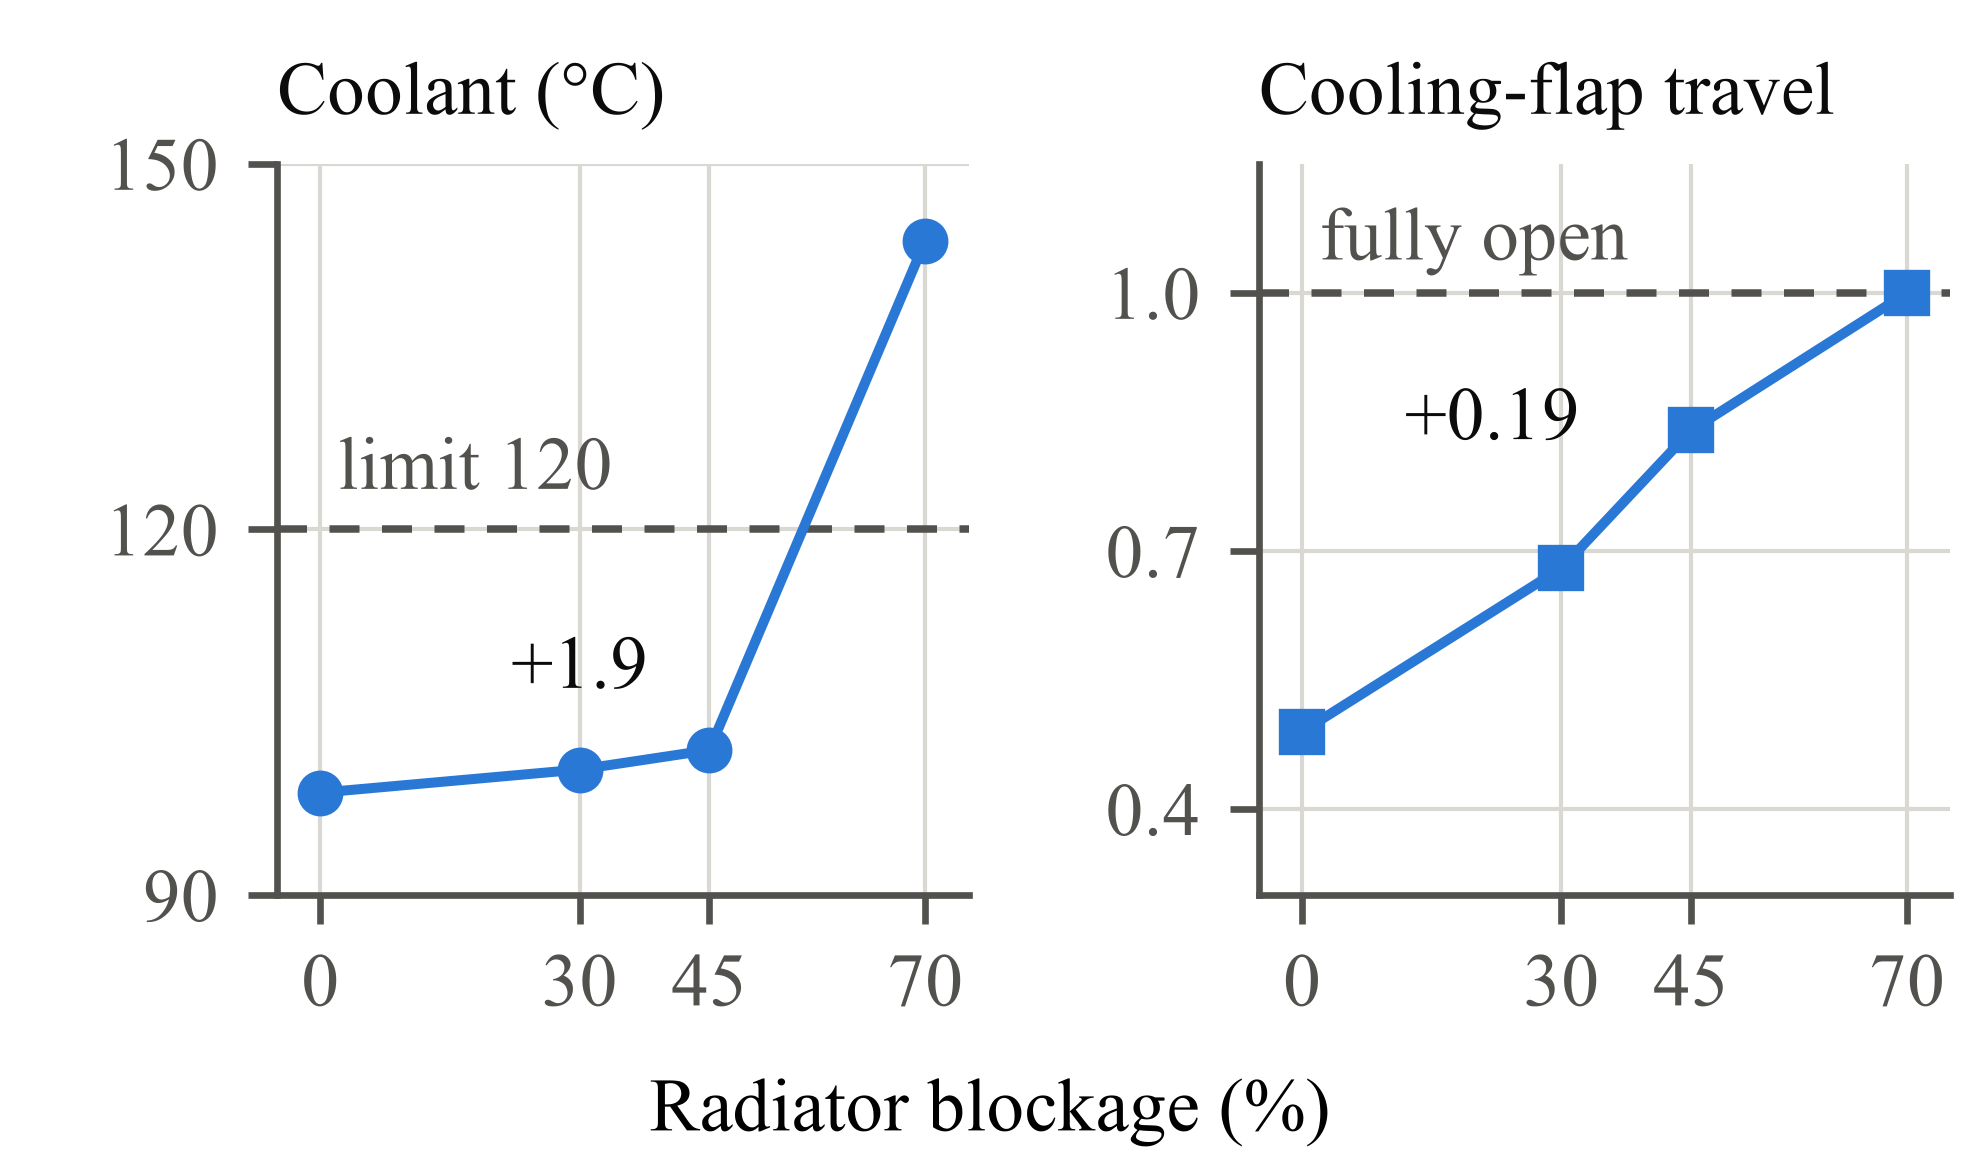
\includegraphics[width=\columnwidth]{figures/fig_cooling.png}
\caption{Why limits are late. Radiator blockage on the shadow twin's test rig at maximum continuous power: coolant temperature rises by only 1.9\,$^\circ$C at 30\% blockage, because the cooling flaps compensate, and crosses its limit only after the flaps are fully open. Flap travel against the twin's as-new expectation exposes the fault while every limit is still satisfied.}
\label{fig:cooling}
\end{figure}

Against 130 full-throttle points from the manufacturer's performance tables, the twin's median absolute errors are 1.05\% for power, 0.43\% for boost pressure, 1.71\% for fuel flow and 0.20\% for engine speed, with 115 of 130 points within 5\% on power. Errors grow to 38--93\% on power at 4,500--5,000~rpm above 15,000~ft, where the model fails to hold the commanded engine speed. Because these tables also informed the model, this is a consistency check of the implementation rather than an independent validation.

\noindent\textbf{Run-to-failure fleet.} A generator flies each virtual engine through sorties of 4--18~h until its composite health index falls below the maintenance threshold of 0.60, or until it reaches the 1,200~h TBO, where it is right-censored. Each engine draws its own manufacturing scatter, operating environment (standard, hot, high-altitude or cold) and rates for six physical degradation pathways, together with faults from eight modes: misfire, injector abnormality, cooling degradation, lubrication issue, sensor drift, combustion instability, overheating trend and abnormal vibration. Faults have random onset and severity and a ramp time set by their physical mechanism, from 0.5--8~h for a misfire to 60--300~h for cooling-jacket fouling. Instruments add noise, bias drift, quantisation and dropouts. Each sortie contributes a fully simulated 50~s window at 1~Hz, and wear is integrated over the rest of the sortie. Labels come from the simulator's internal state; features contain only quantities an aircraft can measure.

We use three versions of the fleet and label every result with its version: \textbf{F100}, 100 engines split 60/20/20 by engine, of which 73 fail before TBO; \textbf{F100-W}, regenerated with condition-dependent (wear-out) fault onset and failure statistics calibrated to match F100, of which 75 fail; and \textbf{F200}, 200 engines split 120/40/40, used for detection and fault naming.

\noindent\textbf{Features and leakage controls.} Each 1~Hz sample carries 34 features: raw channels (engine speed, peak cylinder-head and exhaust temperatures, oil pressure and temperature, fuel flow, vibration), six twin residuals, cylinder-to-cylinder spreads, injection and knock indicators, vibration kurtosis and bearing defect-frequency bands, wastegate and cooling-flap positions with their residuals, and the disagreement between the two redundant control lanes. Manufacturing scatter gives each engine a constant residual offset, so every residual is expressed relative to that engine's own median over its first 60 flight hours, a quantity available in service. Labels and simulator truth (RUL, the censoring flag, engine and sortie identifiers, and all hidden degradation variables) are on a forbidden list enforced in code; the guard rejected one of our own feature sets when a sortie index slipped in. Splits are by engine and stratified by fault composition, so every class appears in validation and test. Thresholds, combiners and calibration are chosen on validation engines, and test engines are scored once. Training and serving share one feature definition and are tested for parity: the deployed RUL path reproduces the training-path metrics to three decimals (2.6~h RMSE between the two predictions).

\noindent\textbf{Footprint.} The deep detector exports to ONNX; INT8 quantisation \citep{jacob2018quant} shrinks it 3.0$\times$ to 55~KB and changed 1 of 300 decisions in a comparison set. One twin update takes 51~ms median and 83~ms at the 95th percentile on an x86-64 PC against a 200~ms budget; we have not yet measured an ARM edge computer.

\section{Point RUL Is Largely Unpredictable}
\label{sec:rul}

\noindent\textbf{Setup.} RUL targets are capped at 400~h, one third of TBO, analogous to the 125-cycle cap used on C-MAPSS; beyond it no maintenance decision changes. We report RMSE in hours, RMSE divided by the standard deviation $\sigma$ of the capped target (1.0 equals predicting the mean), and $\alpha$-$\lambda$ accuracy with $\alpha=0.2$, $\lambda=0.5$ \citep{saxena2010metrics}. Censored windows contribute to training through a one-sided hinge, under which predictions above the censoring bound cost nothing, but are excluded from metrics.

We compare three estimators. \emph{Physics extrapolation} divides the margin of the composite health index above its threshold by a Kalman-filtered rate of decline. The \emph{LSTM} (64 and 32 units with a dense head) reads 30-sample windows of 23 features and is trained with mean squared error plus an asymmetric score that penalises late, over-optimistic predictions more than early ones. The \emph{oracle} is a gradient-boosted regressor on sortie-level hidden state, namely twelve degradation variables and four true health indices, evaluated by engine-grouped 5-fold cross-validation. No sensor can supply more information than this, although the oracle is a strong reference rather than a strict bound.

\begin{table}[t]
\centering
\small
\begin{tabular}{@{}lccc@{}}
\toprule
Estimator & RMSE (h) & RMSE/$\sigma$ & $\alpha$-$\lambda$ \\
\midrule
\multicolumn{4}{@{}l}{\emph{F100, uniform fault onset}} \\
Physics, as served & 226.9 & 1.650 & 0.13 \\
Physics, capped at 400~h & 162.5 & 1.182 & 0.20 \\
LSTM, sensors only & 109.8 & 0.799 & 0.33 \\
Oracle, hidden state & 105.7 & 0.765 & 0.36 \\
Oracle + monotone & \phantom{0}98.1 & 0.710 & 0.36 \\
\midrule
\multicolumn{4}{@{}l}{\emph{F100-W, wear-out fault onset}} \\
LSTM, sensors only & 102.7 & 0.735 & 0.50 \\
LSTM, late-weighted & \phantom{0}95.4 & 0.684 & 0.56 \\
Oracle, hidden state & \phantom{0}99.2 & 0.709 & 0.39 \\
Oracle + monotone & \phantom{0}89.6 & 0.640 & 0.39 \\
\bottomrule
\end{tabular}
\caption{Point RUL. Physics and LSTM rows on F100 are scored on the same 1,914 held-out windows; F100-W LSTM rows use one split of 16 test engines ($\sigma = 139.6$~h); oracle rows use sortie rows under engine-grouped 5-fold cross-validation. Rows are comparable in $\sigma$ units ($\sigma \approx 139$~h), not on identical samples.}
\label{tab:rul}
\end{table}

\noindent\textbf{Results.} Table~\ref{tab:rul} shows the outcome. On F100 the LSTM cuts RMSE by 52\% relative to the physics extrapolation as originally served (226.9 to 109.8~h) and lifts $\alpha$-$\lambda$ from 0.13 to 0.33. Yet it reaches only 0.799$\sigma$, while the oracle, with perfect knowledge of the hidden state, reaches 0.765$\sigma$: the sensor model is within 5\% of it. Even with monotone post-processing, the oracle explains only about half of the variance ($R^2 \approx 0.50$ at 0.710$\sigma$).

A recorded ablation of the same oracle protocol (0.760$\sigma$ in that run) shows where the remaining error lives (Figure~\ref{fig:ceiling}). Even when the oracle is also given the engine's true fault schedule and its true \emph{future} operating profile, it improves only to 0.693$\sigma$. The one feature that collapses the error is the engine's realised whole-life wear rate (0.490$\sigma$), and it is not causal: estimated from the engine's past alone, the same rate brings nothing (0.771$\sigma$), and past and whole-life rates correlate at only $r=0.39$. Faults arrive at random times with random severity and ramp, and they change the rate of decline after the prediction is made, so the information a precise hours estimate needs does not exist at prediction time.

\begin{figure}[t]
\centering
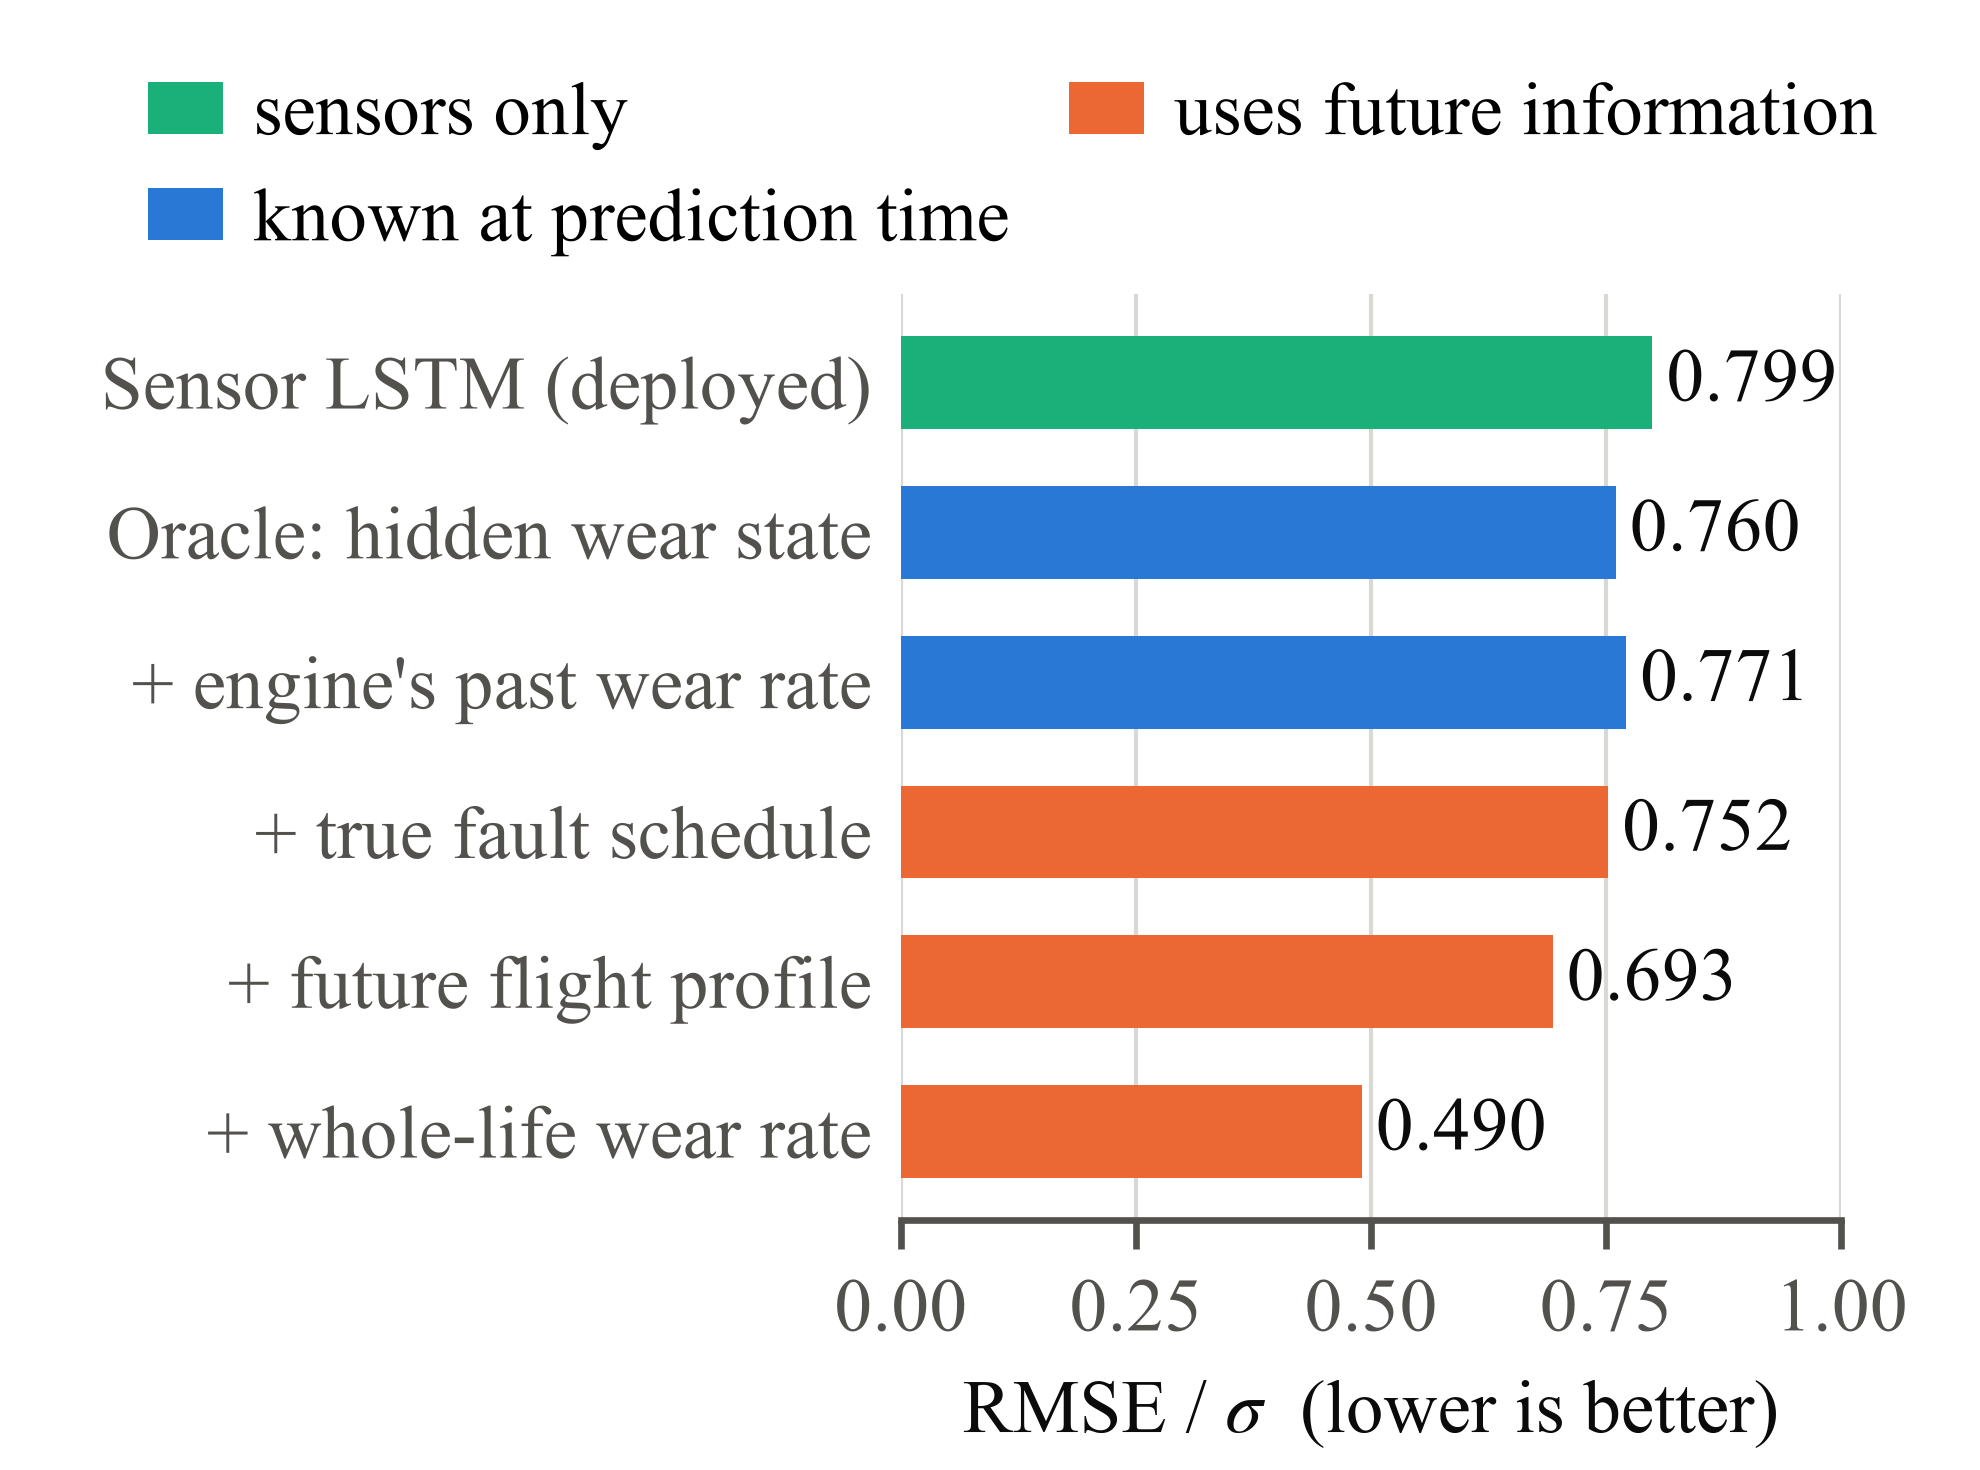
\includegraphics[width=\columnwidth]{figures/fig_ceiling.png}
\caption{How much of point RUL is predictable on F100 (RMSE$/\sigma$; 1.0 equals predicting the mean). Oracles are gradient-boosted regressors on the simulator's hidden state under engine-grouped cross-validation. Each `+' row adds one input to the hidden-state oracle, except that the future-profile row also keeps the fault schedule. Only information from the future reduces the error substantially. The sensor LSTM is scored on held-out windows, so it is comparable in $\sigma$ units only.}
\label{fig:ceiling}
\end{figure}

\noindent\textbf{Wear-out faults.} On F100-W, where fault onset depends on condition, the oracle improves to 0.709$\sigma$ (0.640$\sigma$ monotone) and the LSTM to 0.735$\sigma$; with a heavier penalty on late errors it reaches 0.684$\sigma$, level with the oracle within protocol differences. This confirms that the sensor model extracts most of what is extractable, not that hours became predictable: RMSE is still 95~h on a 140~h spread. Between fleets, the NASA score, which punishes late errors exponentially, rose from 2,252 to 37,964 while the fraction of late predictions stayed at 37\%: the model was late no more often, but much later when it was.

\noindent\textbf{Intervals do not rescue point RUL.} On the 40 held-out F200 engines (15,557 windows), the physics estimator's nominal 95\% interval, propagated from the uncertainty of its fitted rate, covers the truth in only 11.5\% of windows (median width 33~h). A Wiener-process first-passage interval \citep{si2011review} reaches 74\% coverage only by being 952~h wide, most of an engine's life between overhauls.

\section{Calibrated Failure-Horizon Prognostics}
\label{sec:surv}

\noindent\textbf{Formulation.} For sortie $s$ with features $\mathbf{x}_s$ and remaining life $r_s$, we estimate
\begin{equation}
p_H(\mathbf{x}_s) = \Pr(r_s \le H \mid \mathbf{x}_s)
\end{equation}
for $H \in \{12, 25, 50, 100, 200, 400\}$~h, with one classifier per horizon. A full-endurance MALE sortie lasts 12--18~h, so the shortest horizons map onto dispatch decisions and 25--100~h onto maintenance planning. Each sortie is summarised by the level, within-sortie scatter and sortie-to-sortie rate of change of the 34 features, plus flight hours and an estimated health index with its rate (105 features). The classifier is CatBoost \citep{prokhorenkova2018catboost}; in an engine-grouped comparison it matched scikit-learn's histogram gradient boosting and LightGBM within fold noise and was the steadiest at 50~h (Brier-skill standard deviation 0.029, against 0.071 and 0.078).

\noindent\textbf{Calibration and the skill gate.} A probability shown to an operator must mean what it says. We calibrate each horizon with isotonic regression on engines the classifier did not see, in one of two ways: on held-out validation engines, or \emph{out of fold}, pooling predictions from engine-grouped folds over the training and validation engines so that no model is calibrated on rows it was fitted to. We report the Brier skill score $\mathrm{BSS} = 1 - B/B_0$, where $B_0$ is the Brier score of always predicting the base rate. A horizon is shown to operators only if $\mathrm{BSS} \ge 0.05$, and operators are never shown an uncalibrated hours figure.

\noindent\textbf{Censoring.} For an engine withdrawn at TBO, whether it would have failed within $H$ is unknowable near the end of its record. We exclude censored engines from fitting and scoring rather than label them as survivors, which would teach the model that survivors are healthy; Section~\ref{sec:lim} discusses the consequence.

\begin{table*}[t]
\centering
\small
\begin{tabular}{@{}rccccc@{}}
\toprule
 & & \multicolumn{2}{c}{F200 held-out test (1,444 sorties)} & \multicolumn{2}{c}{F100 engine-grouped 6-fold CV (73 engines)} \\
\cmidrule(lr){3-4}\cmidrule(l){5-6}
Horizon $H$ & Base rate & ROC-AUC & Brier skill & ROC-AUC & Brier skill \\
\midrule
12 h & 0.028 & 0.923 & 0.305 & 0.932 $\pm$ 0.026$^\dagger$ & 0.14 $\pm$ 0.13$^\dagger$ \\
25 h & 0.058 & 0.945 & 0.470 & 0.921 $\pm$ 0.033 & 0.40 $\pm$ 0.07 \\
50 h & 0.106 & 0.925 & 0.472 & 0.915 $\pm$ 0.025 & 0.45 $\pm$ 0.03 \\
100 h & 0.199 & 0.899 & 0.523 & 0.891 $\pm$ 0.018 & 0.46 $\pm$ 0.06 \\
200 h & 0.384 & 0.847 & 0.422 & 0.825 $\pm$ 0.045$^\dagger$ & 0.34 $\pm$ 0.10$^\dagger$ \\
400 h & 0.698 & 0.770 & 0.198 & 0.734 $\pm$ 0.061$^\dagger$ & 0.12 $\pm$ 0.08$^\dagger$ \\
\bottomrule
\end{tabular}
\caption{Failure-horizon prognostics. Test columns use CatBoost with out-of-fold isotonic calibration; cross-validation columns give mean $\pm$ standard deviation over folds. $^\dagger$Cross-validated with scikit-learn histogram gradient boosting, the only backend run at these horizons.}
\label{tab:surv}
\end{table*}

\noindent\textbf{Results.} Table~\ref{tab:surv} reports the held-out F200 test engines and engine-grouped 6-fold cross-validation on F100. Discrimination is high at the planning horizons (cross-validated ROC-AUC 0.89--0.92 at 25--100~h), and Brier skill peaks at 50--100~h. Skill decays toward 400~h ($0.12 \pm 0.08$), which is the same far-horizon limit that inflates RMSE, now reported per horizon instead of hidden in an average. At 12~h the ranking is best but skill varies most across folds ($0.14 \pm 0.13$), because only about 3\% of sorties are positive; we treat it as a ranking signal, not yet a calibrated dispatch gate. A single 20-engine split overstated near-horizon AUC by up to 0.05 relative to cross-validation, which is why we quote the grouped figures.

\begin{figure}[t]
\centering
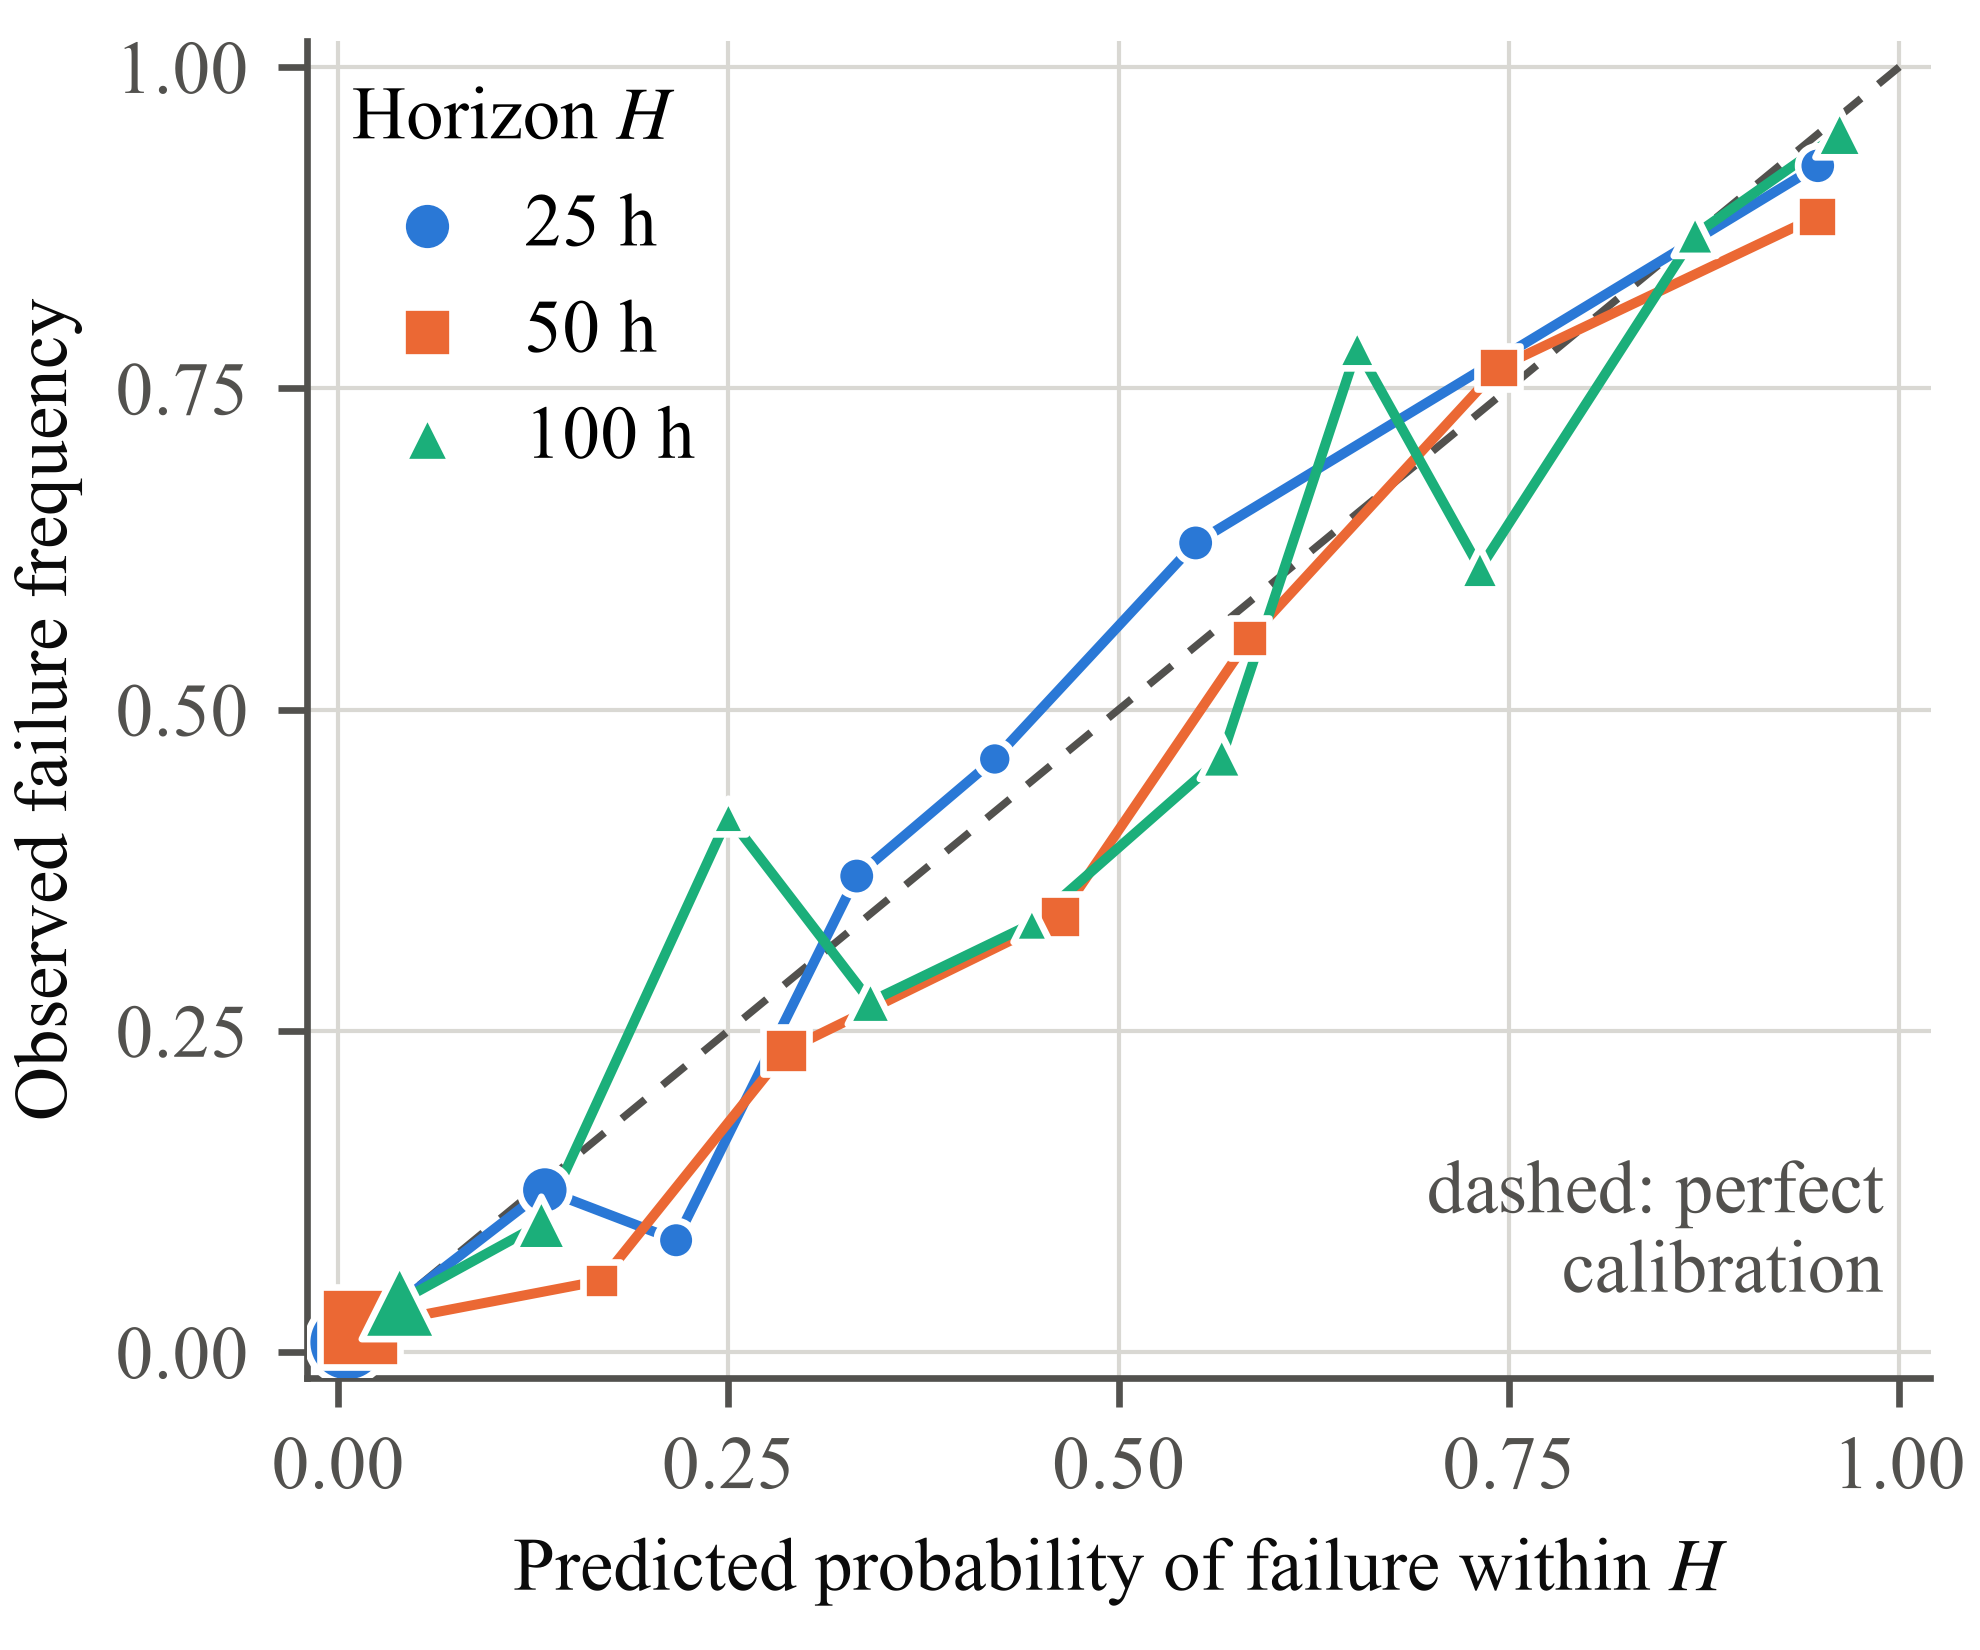
\includegraphics[width=\columnwidth]{figures/fig_reliability.png}
\caption{Reliability of out-of-fold-calibrated failure probabilities on held-out F200 engines (1,444 sorties). Marker area grows with the number of sorties per bin; bins with fewer than 10 sorties are omitted.}
\label{fig:rel}
\end{figure}

Figure~\ref{fig:rel} shows reliability on held-out engines. Compared with validation-set calibration, out-of-fold calibration lowers the n-weighted expected calibration error at each of 12, 25, 50 and 100~h (0.013 to 0.008, 0.009 to 0.007, 0.035 to 0.018 and 0.031 to 0.020) and raises Brier skill from 50~h up (at 100~h, 0.471 to 0.523). Validation-set calibration had issued near-certain 12~h probabilities (mean 0.996) that materialised only 82\% of the time, an error that would ground serviceable aircraft. Some miscalibration remains in mid-range bins, for example 0.46 predicted against 0.34 observed at 50~h ($n=59$).

\section{Safety-Gated Anomaly Detection}
\label{sec:det}

\noindent\textbf{Tiers.} Tier~1 compares validated frames with certified limits, with persistence. Tier~2 is a condition-aware statistical ensemble fitted on healthy training rows: Isolation Forest (100 trees), CBLOF (8 clusters) and a matrix profile (window 100) on the head-temperature residual, weighted 0.4/0.3/0.3 after per-detector score calibration, with thresholds set per operating condition (17 conditions) and a 2-of-3 persistence vote. Tier~3 holds an LSTM autoencoder (32--16--32) and a multi-task LSTM (64 and 32 units) with anomaly, eight-way fault and severity heads, both reading 30-step windows.

\noindent\textbf{Fusion.} With normalised rule level $S_R \in [0,1]$ and calibrated model scores $S_S$ and $S_D$, the reference specification defines $S = 0.3S_R + 0.3S_S + 0.4S_D$ and
\begin{align*}
\textsc{Emergency} &: S > 0.95 \wedge S_R = 1,\\
\textsc{Warning} &: S > 0.80 \wedge (S_S > 0.70 \vee S_D > 0.80),\\
\textsc{Caution} &: S > 0.60 \wedge S_R > 0.50.
\end{align*}
With the rules silent ($S_R = 0$), $S \le 0.70$, so no model finding can ever reach an operator, which is precisely the case the twin exists for. We add one path, $\textsc{Caution}_{\mathrm{pred}}: S_S > 0.70 \wedge S_D > 0.70$, labelled ``developing condition, no limit exceeded'', and an advisory when a single model tier exceeds 0.70. Requiring both model tiers makes the new path depend on two independent methods agreeing. The emergency path is unchanged, so a model can report degradation but cannot declare an emergency on its own. $S_D$ combines the autoencoder and the supervised head; the combiner (mean, maximum, or either alone) is chosen on validation engines by F1, with ties within 0.01 broken by the validation false-alarm rate.

\begin{table}[t]
\centering
\small
\begin{tabular}{@{}lcccc@{}}
\toprule
Detector & AUC & Prec. & Recall & FPR \\
\midrule
Tier 2 statistical & 0.915 & 0.969 & 0.530 & 5.1\% \\
Tier 3 autoencoder & 0.916 & 0.937 & 0.241 & 4.9\% \\
Tier 3 head & 0.962 & 0.983 & 0.936 & 4.9\% \\
Fused, \textsc{Caution}+ & \textbf{0.989} & \textbf{0.996} & 0.870 & \textbf{0.95\%} \\
\bottomrule
\end{tabular}
\caption{Detection on 40 held-out F200 engines (7,635 degraded and 2,525 healthy windows; one engine-grouped split). ROC-AUC is threshold-free; the other columns use each tier's operating threshold, and \textsc{Caution} or above for the fused output.}
\label{tab:det}
\end{table}

\noindent\textbf{Results.} We score 12,165 windows from the 40 held-out F200 engines. A window is \emph{degraded} if a fault is expressed (severity at least 0.2) or the true composite health is at most 0.80, and \emph{healthy} if health is at least 0.90 with no fault above 0.02. The 2,005 windows in between are excluded rather than assigned to whichever class flatters the result. Table~\ref{tab:det} reports each tier and the fused output. Every single tier raises false alarms on about 5\% of healthy windows; fusion cuts that to 0.95\% at precision 0.996 and F1 0.929, paying 6.6 points of recall against the supervised head alone (F1 0.959).

The certified limits fire on only 77 windows, and the specified fusion logic raises 74 alerts. Ours raises 7,256 and catches 6,567 of the 7,558 degraded windows on which every limit is satisfied. Tier~2's deployed rule alone flags all 31 failing test engines a median of 315~h (minimum 63~h) before end of life, at 0.20 false alarms per engine-hour.

\noindent\textbf{Fault naming.} Telling the maintainer \emph{which} fault is present is harder than detecting one. Per-class gradient-boosted classifiers over sortie-history features (running level, scatter and trend across completed sorties, with a sample-only model for an engine's first four sorties) reach macro-F1 0.780 on test engines, against 0.610 for the network's fault head. Misfire (F1 0.97), abnormal vibration (0.94) and lubrication issues (0.93) are named reliably; sensor drift (0.54) and combustion instability (0.46, recall 0.32) are not, because a drifting instrument and uneven combustion both resemble small genuine changes.

\section{External Checks}
\label{sec:ext}

\noindent\textbf{NGAFID.} The National General Aviation Flight Information Database holds 1~Hz flight records from Cessna 172S aircraft with logged unplanned maintenance. We use the benchmark subset of flights within two days of a maintenance event, with its provided five folds \citep{yang2022dataset}, and score per maintenance issue: class 1 is a flight before the event and class 0 a flight after it. We train CatBoost on 46 per-flight features, the level and spread of each channel, which is the same representation as our sortie features. Table~\ref{tab:ngafid} lists the results, with the convolutional models of \citet{yang2022ngafid} as reference points. Those models were trained on a different extraction from the same database (five flights either side of each event), so the comparison is indicative rather than exact. On rocker-cover faults our ROC-AUC (0.764, PR-AUC 0.729) exceeds every Conv-LSTM variant and is within about one standard deviation of the best Conv-MHSA configuration (0.775); on intake-gasket faults (0.772, PR-AUC 0.765) it sits inside the Conv-LSTM range and below Conv-MHSA (0.826). NGAFID records neither vibration nor injection timing, and the Rotax-trained weights are not used, so this checks the representation and method on real faults, not the deployed model.

\begin{table}[t]
\centering
\small
\begin{tabular}{@{}lccc@{}}
\toprule
Issue & Ours & C-LSTM$^\ddagger$ & C-MHSA$^\ddagger$ \\
\midrule
Intake gasket & 0.772 $\pm$ 0.023 & 0.70--0.79 & 0.826 \\
Rocker cover & 0.764 $\pm$ 0.009 & 0.55--0.73 & 0.775 \\
\bottomrule
\end{tabular}
\caption{ROC-AUC on NGAFID (4,310 and 2,260 flights), mean $\pm$ standard deviation over the five provided folds. $^\ddagger$Conv-LSTM range over variants and best Conv-MHSA configuration reported by \citet{yang2022ngafid}, on a different flight extraction.}
\label{tab:ngafid}
\end{table}

\noindent\textbf{C-MAPSS.} To check the RUL network itself, we train the same LSTM on all four C-MAPSS subsets with a 125-cycle cap, 30-cycle windows, per-regime normalisation (k-means over the three operating settings, one scaler per regime, fitted on training units only) and early stopping on a unit-grouped validation split. Over three seeds (Table~\ref{tab:cmapss}) it is better than the LSTM of \citet{zheng2017lstm} on all subsets and better than the DCNN of \citet{li2018dcnn} on the six-regime subsets FD002 and FD004, but worse on FD001 and FD003. Seed-to-seed ranges reach 1.6 RMSE, so differences below that cannot be resolved from a single seed; two of our own earlier single-seed ablation claims did not survive this check and were withdrawn.

\begin{table}[t]
\centering
\small
\begin{tabular}{@{}lccc@{}}
\toprule
Subset & Ours (3 seeds) & LSTM & DCNN \\
\midrule
FD001 & 14.13 $\pm$ 0.66 & 16.14 & 12.61 \\
FD002 & 14.70 $\pm$ 0.49 & 24.49 & 22.36 \\
FD003 & 14.52 $\pm$ 0.62 & 16.18 & 12.64 \\
FD004 & 15.58 $\pm$ 0.31 & 28.17 & 23.31 \\
\bottomrule
\end{tabular}
\caption{Test RMSE (cycles) on C-MAPSS, last cycle per unit. LSTM from \citet{zheng2017lstm} and DCNN from \citet{li2018dcnn}, as reported.}
\label{tab:cmapss}
\end{table}

\section{Limitations}
\label{sec:lim}

\noindent\textbf{Simulated faults.} Every training and test fault comes from our simulator. Stochastic faults, manufacturing scatter, sensor models and engine-level splits reduce, but do not remove, the risk that learned models exploit regularities of the simulator. The twin agrees with the manufacturer's tables at high engine speed but not at 4,500--5,000~rpm above 15,000~ft. Against real Rotax~912 telemetry from NASA's ACES flight campaign (54 flights, 202 steady points; a related but different engine), the as-new twin shows channel offsets of up to 31\,$^\circ$C and residual scatter of up to 77\,$^\circ$C, so per-engine calibration on real hardware will be needed.

\noindent\textbf{Censoring.} Excluding censored engines makes the failure-horizon probabilities conditional on failure before TBO. Keeping censored sorties whose follow-up exceeds $H$, or inverse-probability-of-censoring weighting, is the next step.

\noindent\textbf{Single splits, mixed versions.} Detection and fault-naming results come from one engine-grouped split and one seed, and per-class F1 moved by about 0.10 between training runs. Experiments span three fleet versions, labelled throughout, and latency was measured on x86-64 rather than on the ARM edge target.

\noindent\textbf{Baselines.} We compare the failure-horizon head with point-RUL estimators and with hidden-state oracles, but not yet with survival models such as Cox regression \citep{cox1972} or DeepHit \citep{lee2018deephit} fitted to the same sortie features.

\section{Conclusion}

For a UAV piston engine, an hours-to-failure estimate looks precise but is mostly noise: an oracle with the full hidden state does little better than a sensor model, because the faults that will set the remaining life have not happened yet. Calibrated failure probabilities at planning horizons are both answerable and actionable, and a fusion rule that lets agreeing models warn early while reserving emergencies for crossed limits turns residual-based detection into alerts an operator can trust. Our next steps are censoring-aware training, multi-split error bars for detection, and hardware-in-the-loop tests on a real engine. We intend to release the simulator configuration and evaluation code.
